% =============================================================
% sec05_phuongphap.tex  --  Muc V: Phuong phap nghien cuu (Methodology)
% Bao cao Phase 1 -- Disease-Diagnosis-RAG-System
% Trich dan: who2019icd10, xiao2024cpack, malkov2018hnsw, qwen2025qwen3
% =============================================================

\section{Phương pháp nghiên cứu (Methodology)}
\label{sec:phuongphap}

\subsection{Tổng quan pipeline hai tầng (Two-Layer RAG)}

Thiết kế A (DDXPlus-only, \textit{retrieval-first}) bao gồm năm giai đoạn. Đầu tiên, \textbf{Knowledge Base (KB)} được xây dựng từ định nghĩa bệnh và các bằng chứng (evidence) sau khi được tiền xử lý và chuẩn hoá bằng các kỹ thuật NLP. Tiếp theo, KB được \textbf{lập chỉ mục} trên OpenSearch với hai loại chỉ mục: chỉ mục từ vựng phục vụ BM25 và chỉ mục vector phục vụ truy xuất k-NN.

Ở giai đoạn \textbf{truy xuất}, hệ thống hỗ trợ ba chiến lược: BM25 (lexical retrieval), Dense Retrieval (semantic retrieval dựa trên embedding và độ tương đồng cosine) và Hybrid Retrieval, trong đó kết quả của BM25 và Dense được hợp nhất bằng kỹ thuật Reciprocal Rank Fusion (RRF). Các tài liệu top-$K$ sau truy xuất được đưa qua bước \textbf{re-ranking} bằng cross-encoder nhằm cải thiện chất lượng xếp hạng. Thành phần này đã được hiện thực trong Phase~1 nhưng chỉ được đánh giá định lượng ở Phase~2. Cuối cùng, các tài liệu đã được xếp hạng sẽ được sử dụng làm ngữ cảnh để \textbf{sinh câu trả lời} bằng LLM trong Phase~2.

Để tách biệt chất lượng của thuật toán truy xuất khỏi ảnh hưởng của hạ tầng triển khai, mỗi chiến lược được đánh giá trên hai môi trường thực thi song song: (i) chế độ \textit{offline} (in-memory, bằng Python thuần) làm mốc tham chiếu và (ii) hệ thống OpenSearch, sử dụng các cơ chế lập chỉ mục và truy xuất tương ứng trong môi trường triển khai thực tế.

\begin{figure}[H]
    \centering
    \resizebox{\textwidth}{!}{%
        \begin{tikzpicture}[node distance=0.9cm]
            \node[stage, text width=2.1cm] (q) {Truy vấn bệnh nhân\\(EVIDENCES + tuổi/giới)};
            \node[stage, text width=2.0cm, right=of q] (pre) {Tiền xử lý\\decode + chuẩn hoá};
            \node[stage, text width=2.5cm, right=of pre] (hyb) {Truy xuất Hybrid\\BM25 (keyword\_text) + k-NN (BGE 384-d)};
            \node[stage, text width=1.9cm, right=of hyb] (rrf) {RRF $k=60$\\$\rightarrow$ top-20};
            \node[future, text width=1.9cm, right=of rrf] (rr) {Re-ranking\\top-20 $\rightarrow$ top-5\\(Phase 2)};
            \node[future, text width=1.9cm, right=of rr] (gen) {Sinh câu trả lời\\Qwen3-8B\\(Phase 2)};
            \draw[flow] (q) -- (pre);
            \draw[flow] (pre) -- (hyb);
            \draw[flow] (hyb) -- (rrf);
            \draw[flow] (rrf) -- (rr);
            \draw[flow] (rr) -- (gen);
        \end{tikzpicture}}
    \caption{Pipeline RAG hai tầng (Thiết kế A). Khối nét liền: hoàn thiện và đánh giá ở Phase 1. Khối nét đứt: re-ranking (mã nguồn hoàn thiện ở cuối Phase 1, đánh giá định lượng ở Phase 2) và sinh câu trả lời (Phase 2).}
    \label{fig:pipeline}
\end{figure}

\subsection{Từ dữ liệu thô đến Knowledge Base: quy trình NLP}

Knowledge Base (KB) được xây dựng thông qua kịch bản \texttt{scripts/build\_kb.py}, đảm nhiệm vai trò chuyển đổi dữ liệu thô thành phiên bản chuẩn hoá phục vụ cho khâu truy xuất. Toàn bộ quá trình chuẩn hoá sử dụng chung mô-đun tiền xử lý \texttt{src/services/rag/preprocess.py} cho cả hai giai đoạn: xây dựng chỉ mục (ingest) và xử lý truy vấn (query), qua đó bảo đảm văn bản được chuẩn hoá nhất quán giữa thời điểm lập chỉ mục và thời điểm truy xuất.

\paragraph{(a) Nguồn dữ liệu và trích xuất trường.}
Knowledge Base được xây dựng từ hai tệp của bộ dữ liệu DDXPlus: \texttt{release\_conditions.json} (49 bệnh) và \texttt{release\_evidences.json} (223 evidence). Đối với mỗi bệnh, hệ thống trích xuất các trường cốt lõi gồm tên bệnh (\texttt{cond-name-eng}), danh sách evidence trong \texttt{symptoms} và \texttt{antecedents}, mức độ nghiêm trọng (\texttt{severity}, trên thang điểm từ 1 đến 5) và mã ICD-10 (\texttt{icd10-id}).

\paragraph{(b) Chuẩn hoá cụm triệu chứng (\texttt{normalize\_symptom\_phrase}).}
Mỗi mã evidence được ánh xạ sang câu hỏi tiếng Anh (\texttt{question\_en}) rồi chuyển đổi thành một cụm danh từ biểu diễn triệu chứng thông qua hàm \texttt{normalize\_symptom\_phrase}. Quy trình chuẩn hoá bao gồm các bước sau:
\begin{enumerate}[leftmargin=1.4em,itemsep=2pt]
    \item Áp dụng \textbf{bảng ghi đè (override table)} cho các câu hỏi đặc biệt không thể xử lý chính xác bằng các quy tắc tổng quát. Bảng này gồm 24 phép ánh xạ được xây dựng thủ công nhằm bảo toàn ý nghĩa lâm sàng. Ví dụ, \textit{``Characterize your pain:''} được chuyển thành \texttt{pain character}, \textit{``Have you traveled out of the country in the last 4 weeks?''} thành \texttt{recent international travel}, và \textit{``Do you have a cough?''} thành \texttt{cough}.
    \item Chuẩn hoá văn bản bằng cách chuyển toàn bộ về chữ thường, loại bỏ khoảng trắng dư thừa, nội dung nằm trong dấu ngoặc và các dấu câu ở cuối.
    \item Loại bỏ các mẫu mở đầu của câu hỏi (\texttt{\_LEAD\_FRAMES}), chẳng hạn như \textit{``Do you have''}, \textit{``Have you ever''} hoặc \textit{``Are you''}, nhằm cô đọng lại phần nội dung mang ý nghĩa lâm sàng.
    \item Loại bỏ các mệnh đề nối và từ chức năng không mang giá trị thông tin (ví dụ: \textit{been}, \textit{had}, \textit{a}, \textit{the}, \textit{with}, \textit{to}), sau đó chuẩn hoá khoảng trắng để thu được cụm triệu chứng hoàn chỉnh cuối cùng.
\end{enumerate}
Quy trình trên giúp chuyển đổi các câu hỏi mang tính hội thoại trong DDXPlus thành các cụm triệu chứng ngắn gọn, nhất quán, góp phần cải thiện hiệu quả lập chỉ mục và truy xuất. Trước bước này, \texttt{PreprocessPipeline} còn thực hiện \textbf{mở rộng từ đồng nghĩa} (ví dụ: \textit{tired/exhausted} $\rightarrow$ \texttt{fatigue}, \textit{throwing up} $\rightarrow$ \texttt{vomiting}). Các triệu chứng và tiền sử sau khi chuẩn hoá được \textbf{khử trùng lặp nhưng vẫn giữ nguyên thứ tự}.

\paragraph{(c) Chuẩn hoá mã ICD-10~\cite{who2019icd10} và định danh tài liệu.}
Mã ICD-10 được chuẩn hoá thông qua hàm \texttt{normalize\_icd10}, bao gồm việc chuyển sang chữ in hoa và loại bỏ khoảng trắng thừa. Đối với các bệnh có nhiều mã ICD-10, hệ thống tiến hành tách từng mã riêng biệt bằng hàm \texttt{split\_icd10\_codes} trước khi xác định \texttt{doc\_id}. Mỗi tài liệu được gán một \texttt{doc\_id} duy nhất theo quy tắc tất định nhằm bảo đảm tính toàn vẹn trong quá trình lập chỉ mục và truy xuất. Một số trường hợp ngoại lệ được tinh chỉnh bằng bảng override; ví dụ, bệnh \textit{Pneumonia} có cặp mã \texttt{(J17, J18)} được ánh xạ về \texttt{J18} làm \texttt{doc\_id} chuẩn.

\paragraph{(d) Sinh các trường dẫn xuất.}
Từ ba trường thông tin gốc gồm tên bệnh (\textit{disease}), triệu chứng (\textit{symptoms}) và tiền sử (\textit{antecedents}), hệ thống tổng hợp thêm các trường mới để phục vụ truy xuất và sinh câu trả lời:
\begin{itemize}[leftmargin=1.4em,itemsep=2pt]
    \item \texttt{keyword\_text}: chuỗi ghép nối của \textit{disease}, \textit{symptoms} và \textit{antecedents}, được dùng để lập chỉ mục cho việc truy xuất từ vựng bằng thuật toán BM25.
    \item \texttt{embedding}: vector biểu diễn 384 chiều được sinh ra bởi mô hình BGE~\cite{xiao2024cpack} từ chuỗi định dạng \texttt{"Disease: ... Symptoms: ... Antecedents: ..."}, sau đó chuẩn hoá L2 và lưu trữ trong chỉ mục vector để phục vụ Dense Retrieval.
    \item \texttt{description}: mô tả dưới định dạng \texttt{"Condition characterized by: ... Risk factors: ..."}. Trong cấu hình mặc định, trường này không tham gia vào quá trình tạo embedding mà chỉ đóng vai trò làm ngữ cảnh cho LLM ở Phase~2. Tuy nhiên, ảnh hưởng của việc bổ sung \texttt{description} vào \texttt{keyword\_text} (cho BM25) và vào chuỗi sinh embedding (cho Dense Retrieval) đã được khảo sát thực nghiệm và phân tích riêng tại mục Kết quả và Ablation.
    \item metadata bao gồm \texttt{doc\_id}, \texttt{severity} và \texttt{source}.
\end{itemize}

\paragraph{(e) Kiểm định tính nhất quán.}
Sau khi xây dựng Knowledge Base, hệ thống thực hiện loạt kiểm tra tự động nhằm bảo đảm tính toàn vẹn của dữ liệu, bao gồm: xác nhận chính xác 49 tài liệu, bảo đảm \texttt{doc\_id} là duy nhất, \texttt{severity} nằm trong khoảng $[1,5]$ và vector embedding có kích thước đúng chuẩn. Nhóm duy trì song song hai phiên bản KB: bản đã chuẩn hoá (\texttt{kb\_ddxplus.json}) và bản giữ nguyên câu hỏi gốc (\texttt{kb\_ddxplus\_rawq.json}) để tiện cho việc đánh giá ảnh hưởng của bước tiền xử lý. Kết quả rà soát (thể hiện trong \href{https://github.com/AIVIETNAM-AIO-Lucyna/Disease-Diagnosis-RAG-System/pull/6}{PR~\#6}) đã xác nhận không còn sự sai lệch về token giữa dữ liệu nguồn và dữ liệu sau xử lý, đảm bảo sự tương thích tuyệt đối giữa giai đoạn xây dựng chỉ mục và truy xuất.

\subsection{Vì sao chọn OpenSearch}
Bài toán truy xuất trong nghiên cứu này đặt ra yêu cầu phải hỗ trợ đồng thời ba chiến lược trên cùng một Knowledge Base: truy xuất từ vựng (BM25), truy xuất vector (Dense Retrieval) và truy xuất kết hợp (Hybrid Retrieval). Thay vì triển khai và duy trì nhiều hệ thống cơ sở dữ liệu riêng lẻ, nghiên cứu lựa chọn OpenSearch vì nền tảng này hỗ trợ toàn diện cả ba cơ chế trong một hệ sinh thái thống nhất, giúp tinh gọn kiến trúc hệ thống và bảo đảm sự đồng bộ giữa các luồng truy xuất.
\begin{itemize}[leftmargin=1.4em,itemsep=2pt]
    \item \textbf{BM25}: được hỗ trợ trực tiếp thông qua trường dữ liệu kiểu \texttt{text} (cụ thể là \texttt{keyword\_text}) và truy vấn \texttt{match}.
    \item \textbf{Dense Retrieval}: khai thác trường \texttt{knn\_vector} (384 chiều) kết hợp với độ đo tương đồng cosine để thực thi việc tìm kiếm vector lân cận xấp xỉ (Approximate Nearest Neighbor).
    \item \textbf{Hybrid Retrieval}: kết hợp điểm số của BM25 và Dense Retrieval thông qua truy vấn \texttt{hybrid}, sau đó hợp nhất thứ hạng tự động bằng \emph{Reciprocal Rank Fusion} (RRF) ngay trong search pipeline mà không cần hiện thực cơ chế fusion ở tầng ứng dụng.
    \item \textbf{Triển khai thực tế}: nền tảng hỗ trợ nạp dữ liệu hàng loạt (\emph{bulk ingest}), khai báo sơ đồ dữ liệu (mapping) minh bạch, và đặc biệt là cơ chế bí danh alias (\texttt{diseases}), cho phép thay thế chỉ mục (\emph{index swapping}) mà không làm gián đoạn dịch vụ.
\end{itemize}
Sử dụng OpenSearch cho phép toàn bộ pipeline production vận hành trên một cơ sở hạ tầng duy nhất, đồng thời tạo điều kiện đối chiếu khách quan với harness đánh giá offline (do cả hai đều sử dụng chung một KB và quy trình tiền xử lý). Nhờ vậy, những chênh lệch về hiệu năng quan sát được trong thực nghiệm sẽ phản ánh chân thực năng lực của bản thân thuật toán thay vì bị nhiễu bởi yếu tố hạ tầng. Ba thành phần hạ tầng cốt lõi được minh hoạ lần lượt dưới đây: mapping chỉ mục (Hình~\ref{fig:os-mapping}), alias \texttt{diseases} phục vụ hoán đổi chỉ mục (Hình~\ref{fig:os-alias}) và search pipeline RRF (Hình~\ref{fig:os-pipeline}).

\begin{figure}[H]
    \centering
    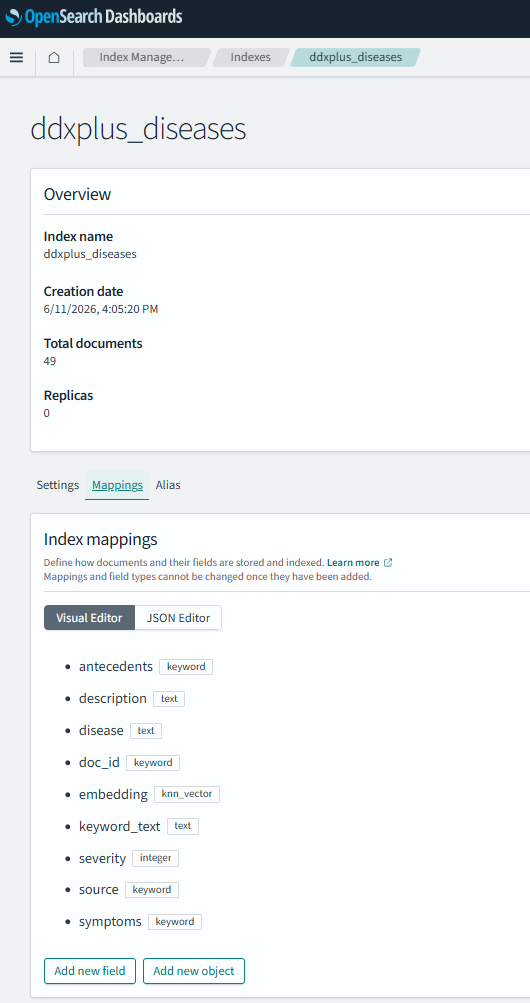
\includegraphics[width=0.42\textwidth]{Figures/ddxplus_mapping.png}
    \caption{Mapping chỉ mục \texttt{ddxplus\_diseases}: trường \texttt{keyword\_text} (\texttt{text}) phục vụ BM25, trường \texttt{embedding} (\texttt{knn\_vector}, 384 chiều, \texttt{cosinesimil}) phục vụ k-NN, đi kèm các metadata như \texttt{doc\_id}, \texttt{severity}, \texttt{description}\dots}
    \label{fig:os-mapping}
\end{figure}

\begin{figure}[H]
    \centering
    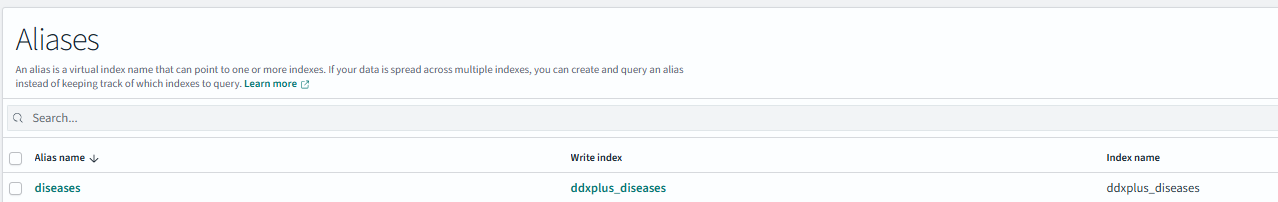
\includegraphics[width=0.95\textwidth]{Figures/alias.png}
    \caption{Bí danh (Alias) \texttt{diseases} trỏ tới chỉ mục vật lý hiện hành, cho phép \textit{swap} chỉ mục khi tiến hành tái lập (reindex) mà không làm rớt các yêu cầu truy vấn.}
    \label{fig:os-alias}
\end{figure}

\begin{figure}[H]
    \centering
    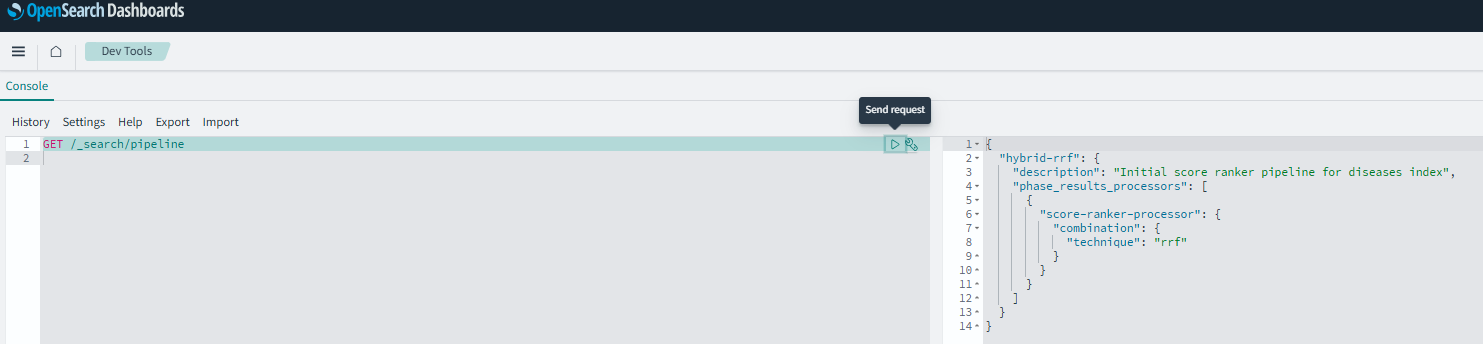
\includegraphics[width=0.95\textwidth]{Figures/phase_result_processor.png}
    \caption{Search pipeline \texttt{hybrid-rrf} tích hợp \texttt{score-ranker-processor} (sử dụng kỹ thuật \texttt{rrf}): hợp nhất thứ hạng của nhánh lexical (BM25) và nhánh semantic (k-NN) trực tiếp bên trong search engine.}
    \label{fig:os-pipeline}
\end{figure}

\subsection{Các chiến lược truy xuất: công thức và tham số}

\paragraph{BM25 (Okapi).}
BM25 được lựa chọn làm mô hình truy xuất từ vựng cốt lõi. Điểm số phù hợp giữa một truy vấn $Q$ và một tài liệu $D$ được định lượng theo công thức:
\begin{equation}
    \mathrm{BM25}(Q,D)=\sum_{t\in Q}\mathrm{IDF}(t)
    \cdot
    \frac{f(t,D)\,(k_1+1)}
    {f(t,D)+k_1\!\left(1-b+b\,\dfrac{|D|}{\mathrm{avgdl}}\right)},
\end{equation}
với thành phần tần số tài liệu nghịch đảo (IDF) được tính bằng:
\[
    \mathrm{IDF}(t)=
    \ln\!\left(
    1+\frac{N-n(t)+0.5}{n(t)+0.5}
    \right),
\]
trong đó $f(t,D)$ là tần suất xuất hiện của từ $t$ trong tài liệu, $|D|$ là độ dài tài liệu, $\mathrm{avgdl}$ là độ dài trung bình của toàn bộ tập tài liệu, $N$ đại diện cho tổng số tài liệu và $n(t)$ là số lượng tài liệu có chứa từ $t$.
Trong thiết lập thực nghiệm, hệ thống offline cấu hình BM25 với tham số $k_1=1.5$, $b=0.75$ kết hợp tokenizer \texttt{[a-z0-9]+}. Ngược lại, hệ thống production sử dụng cấu hình BM25 mặc định của OpenSearch ($k_1=1.2$, $b=0.75$) cùng với \textit{standard analyzer} trên trường \texttt{keyword\_text}. Truy vấn \texttt{match} được thực thi với toán tử \texttt{OR} (tài liệu được cộng điểm nếu chứa bất kỳ từ khoá nào có trong truy vấn). Hiệu năng của BM25 được đánh giá qua hai biến thể: truy vấn trên trường \texttt{keyword\_text} độc lập, và truy vấn trên trường \texttt{keyword\_text} kết hợp \texttt{description} (chi tiết xem tại mục Kết quả).

\paragraph{Dense Retrieval (k-NN).}
Dense Retrieval khai thác năng lực của mô hình \texttt{BAAI/bge-small-en-v1.5}~\cite{xiao2024cpack} để mã hoá cả truy vấn lẫn tài liệu thành không gian vector 384 chiều. Mức độ tương đồng về ngữ nghĩa được xác định qua hàm cosine:
\begin{equation}
    \mathrm{sim}(q,d)=\cos(\mathbf{v}_q,\mathbf{v}_d)
    =\frac{\mathbf{v}_q\cdot\mathbf{v}_d}
    {\lVert\mathbf{v}_q\rVert\,\lVert\mathbf{v}_d\rVert}.
\end{equation}
Vector của các tài liệu (đã được \textbf{chuẩn hoá L2}, do đó phép tính cosine tương đương với tích vô hướng dot-product) được sinh ra từ chuỗi ghép nối tên bệnh, triệu chứng và tiền sử trong khâu xây dựng KB. Hệ thống truy xuất production vận hành trên chỉ mục \texttt{knn\_vector} của OpenSearch (với cấu hình \texttt{space\_type=cosinesimil}, \texttt{index.knn=true}), sử dụng thuật toán tìm kiếm xấp xỉ HNSW~\cite{malkov2018hnsw} do engine Lucene cung cấp (tham số \texttt{ef\_construction}=100, \texttt{m}=16). Với quy mô Knowledge Base rất nhỏ chỉ gồm 49 tài liệu, kết quả tìm kiếm xấp xỉ gần như tiệm cận hoàn toàn với tìm kiếm vét cạn chính xác (exact k-NN); ưu thế về tốc độ của thuật toán HNSW chỉ thực sự phát huy khi quy mô tài liệu lớn hơn đáng kể. Số lượng lân cận truy xuất mặc định được thiết lập là $k=20$.

Điểm khác biệt trọng yếu giữa hai chế độ đánh giá (offline vs. production) nằm ở \textbf{cách biểu diễn chuỗi truy vấn} (tham khảo thêm về cách dùng tiền tố của họ mô hình BGE tại~\cite{xiao2024cpack}). Cụ thể: môi trường offline dựng chuỗi truy vấn dưới dạng câu tự nhiên \texttt{"Symptoms and antecedents: \dots"} và tiến hành mã hoá \textit{không} sử dụng tiền tố (prefix). Trong khi đó, môi trường production dùng hàm \texttt{embed\_query()} nối trực tiếp các token đã chuẩn hoá và gắn thêm tiền tố định hướng của BGE (\texttt{"Represent this sentence for searching relevant passages:"}). Sự bất đối xứng giữa truy vấn và tài liệu này được phân tích như nguyên nhân chính gây chênh lệch hiệu năng Dense Retrieval giữa hai chế độ ở mục Thảo luận.

\paragraph{Hybrid Retrieval (Reciprocal Rank Fusion).}
Hybrid Retrieval thực hiện việc phối hợp kết quả từ hai hướng truy xuất (BM25 và Dense Retrieval) dựa trên phương pháp \textit{Reciprocal Rank Fusion} (RRF):
\begin{equation}
    \mathrm{RRF}(d)=
    \sum_{r\in\{\mathrm{BM25},\,\mathrm{Dense}\}}
    \frac{1}{k+\mathrm{rank}_r(d)},
    \qquad
    k=60.
\end{equation}
Thay vì phải tìm cách chuẩn hoá và cộng gộp các thang điểm số (vốn rất khác biệt về mặt bản chất toán học giữa BM25 và Cosine), thuật toán RRF chỉ quan tâm đến \textit{vị trí thứ hạng} của tài liệu trong từng danh sách trả về, và \textbf{gán trọng số bằng nhau} cho cả nhánh BM25 lẫn Dense. Hằng số điều chuẩn $k=60$ là cấu hình mặc định của \texttt{score-ranker-processor}. Hệ thống offline tự thực hiện tính toán RRF trên hai mảng danh sách kết quả cục bộ, trong khi hệ thống production sử dụng truy vấn \texttt{hybrid} tích hợp \texttt{score-ranker-processor} gốc của OpenSearch. Cả hai hệ thống đều thiết lập trả về top-20 tài liệu.

\paragraph{Re-ranking và sinh câu trả lời.}
Bước sang Phase~2, 20 tài liệu được truy xuất sẽ trải qua khâu sắp xếp lại (re-ranking) bằng mô hình cross-encoder \texttt{bge-reranker-base}~\cite{xiao2024cpack}. Khác với kiến trúc bi-encoder (mã hoá truy vấn và tài liệu một cách \textit{độc lập} rồi mới tính toán khoảng cách cosine), kiến trúc cross-encoder sẽ \textbf{mã hoá đồng thời toàn bộ cặp (truy vấn, tài liệu)} xuyên qua một mạng Transformer. Quá trình này giúp mô hình nắm bắt tương tác chéo (cross-attention) mức từ vựng, mang lại điểm liên quan chính xác hơn, sau đó hệ thống giữ lại top-5 tài liệu cuối cùng (\texttt{RERANK\_TOP\_K}$=5$). Các tài liệu này được dùng làm ngữ cảnh truyền vào mô hình ngôn ngữ \texttt{Qwen3-8B}~\cite{qwen2025qwen3} để sinh ra câu trả lời tự nhiên. Tại thời điểm báo cáo, mã nguồn cho phần re-ranking đã hoàn tất, nhưng việc phân tích và đánh giá các chỉ số định lượng liên quan được lên kế hoạch cho Phase~2.

\subsection{Hai chế độ đánh giá: in-memory offline và OpenSearch production}

Với mục tiêu đánh giá khách quan chất lượng của các chiến lược truy xuất, đồng thời tách biệt ảnh hưởng của hạ tầng triển khai, nhóm nghiên cứu đã thiết lập hai bộ khai thác (harness) chạy song song trên cùng một Knowledge Base, dùng chung một pipeline tiền xử lý và đo lường trên cùng một bộ dữ liệu gán nhãn. Hai chế độ này chỉ khác biệt về lõi thực thi (execution engine), được tóm tắt chi tiết trong Bảng~\ref{tab:harness}.

\begin{enumerate}[leftmargin=1.4em,itemsep=2pt]
    \item \textbf{Offline (in-memory).} Toàn bộ logic truy xuất được lập trình và chạy hoàn toàn bằng Python, độc lập hoàn toàn với OpenSearch. BM25 được cài đặt bám sát công thức lý thuyết Okapi ($k_1=1.5$, $b=0.75$), Dense Retrieval sử dụng thư viện \texttt{sentence-transformers} nạp mô hình \texttt{BAAI/bge-small-en-v1.5}~\cite{xiao2024cpack}, và Hybrid Retrieval tính toán RRF ($k=60$) thủ công. Do Knowledge Base có quy mô nhỏ (49 tài liệu), việc tính toán brute-force trên toàn bộ tập dữ liệu có chi phí tính toán thấp, đủ để làm mốc tham chiếu cho chất lượng của các thuật toán truy xuất.
    \item \textbf{Production (OpenSearch).} Knowledge Base được nạp (ingest) thực tế vào OpenSearch thông qua API, trải qua quy trình chuẩn hoá, sinh vector và bulk indexing thực thụ. Các tác vụ tìm kiếm được gọi qua giao thức RESTful sử dụng \texttt{match} (BM25), \texttt{knn} (Dense) và \texttt{hybrid} (RRF pipeline). Đây chính là mô hình phản ánh đúng cấu hình của hệ thống production đang chạy phục vụ người dùng cuối.
\end{enumerate}

\paragraph{Xây dựng truy vấn và nhãn đánh giá.}
Chuỗi truy vấn của mỗi bệnh nhân được xây dựng từ trường \texttt{EVIDENCES} thông qua các bước làm sạch nghiêm ngặt: cắt bỏ các hậu tố giá trị cụ thể (\texttt{\_@\_<value>}), ánh xạ từng mã hệ thống thành cụm từ y khoa thông qua hàm \texttt{normalize\_symptom\_phrase}, khử trùng lặp và cuối cùng là nối thành câu truy vấn. Tên của bệnh (chẩn đoán cuối cùng) bị loại bỏ hoàn toàn khỏi truy vấn để ngăn chặn triệt để hiện tượng rò rỉ dữ liệu nhãn (data leakage). Nhãn đúng được lấy từ trường \texttt{PATHOLOGY} của bộ dữ liệu gốc DDXPlus.

\paragraph{Chỉ số đánh giá.}
Hệ thống sử dụng một bộ các chỉ số đo lường học thuật tiêu chuẩn trong Information Retrieval, bao gồm Hit@1, Hit@3, Hit@5 và Mean Reciprocal Rank (MRR), trong đó Hit@1 được định vị là chỉ số tối quan trọng (primary metric). Bản chất toán học của chúng như sau:
\begin{itemize}[leftmargin=1.4em,itemsep=2pt]
    \item \textbf{Hit@$k$} (Tỉ lệ trúng đích trong top-$k$): Trả về giá trị nhị phân $1$ nếu tài liệu chứa bệnh lý kỳ vọng nằm gọn trong top $k$ tài liệu trả về đầu tiên, ngược lại nhận giá trị $0$. Giá trị tổng quát được tính bằng giá trị trung bình trên toàn bộ tập truy vấn. \textbf{Hit@1} đánh giá năng lực dự đoán trúng đích ở ngay vị trí số 1 (mô phỏng tình huống hệ thống tự động đưa ra một chẩn đoán duy nhất). \textbf{Hit@3} và \textbf{Hit@5} thể hiện khả năng hệ thống cung cấp một danh sách ngắn gọn nhưng chứa đựng chẩn đoán đúng để bác sĩ chuyên môn tiến hành loại trừ (differential diagnosis).
    \item \textbf{MRR} (Mean Reciprocal Rank): Là trung bình cộng của nghịch đảo thứ hạng ($1/\mathrm{rank}$) của tài liệu chứa bệnh đúng đối với mọi truy vấn. (Trường hợp tài liệu đúng hoàn toàn không xuất hiện, giá trị nghịch đảo bằng $0$). Không giống Hit@$k$ chỉ mang tính nhị phân "có/không", MRR là một chỉ số liên tục, thưởng điểm cao hơn khi tài liệu đúng đứng ở \textit{những vị trí càng cao}, do đó nó nhạy hơn trong việc phản ánh chất lượng xếp hạng tinh hơn. Trong nghiên cứu này, MRR được tính trượt trên toàn vẹn 49 tài liệu (không bị áp dụng cắt tỉa ngưỡng top-$k$).
\end{itemize}
Mặt khác, do không gian đáp án chỉ gói gọn trong 49 tài liệu, đường cơ sở xác suất nếu chọn ngẫu nhiên (random guess baseline) của các chỉ số này (với Hit@1 $\approx 2\%$) sẽ được làm rõ hơn trong phần Dữ liệu và thiết lập thí nghiệm.